\documentclass[10pt,twocolumn]{article}

% ---------------------------------------------------------
% Packages
% ---------------------------------------------------------
\usepackage[utf8]{inputenc}
\usepackage[T1]{fontenc}
\usepackage{lmodern}

\usepackage[margin=0.75in]{geometry}
\usepackage{microtype}

\usepackage{graphicx}
\usepackage{placeins}
\usepackage{booktabs}
\usepackage{array}

\usepackage{amsmath}
\usepackage{amssymb}
\usepackage{mathtools}

\usepackage{enumitem}
\usepackage{xcolor}

\usepackage[numbers,sort&compress]{natbib}
\usepackage[hidelinks]{hyperref}

% ---------------------------------------------------------
% Paper metadata
% ---------------------------------------------------------
\title{
\textbf{Guardian Lens: Controlled Black-Box Identification of\\
Visual-Conditional Decision Policies in a Vision-Language Model}
}

\author{
Mostafa Bdeir, Mohammad Kassira
}

\date{}

% ---------------------------------------------------------
% Document
% ---------------------------------------------------------
\begin{document}

\maketitle

\begin{abstract}

Can a black-box auditor recover which of several controlled decision
policies generated a vision-language model's behavior? Guardian Lens
studies this question using three researcher-induced profiles---Neutral, visual Cue-bound, and Generalized---in a vision-language model whose weights
we do not modify. The benchmark combines matched visual
counterfactuals, quantitative allocation decisions under explicit
counter-incentives, and a transparent behavioral classifier calibrated
before held-out evaluation.

A nearest-centroid auditor was constructed from six calibration scenes
and frozen before evaluation on 12 held-out scenes comprising 432
blinded model calls. It recovered 33 of 36 scene-profile blocks,
yielding 91.7\% accuracy and macro-F1 = 0.915. Cue-bound target-emblem
effects exceeded Neutral behavior by 38.15 allocation points, while
Generalized prioritization persisted under the primary 20\% efficiency
penalty. All three classification errors occurred on distractor scenes
and took the same form, Cue-bound \(\rightarrow\) Neutral, exposing a
specific observability boundary when the conditional policy's activation
condition is absent.

A separate pre-specified 1,296-call cost-response extension varied the
efficiency penalty for favoring Organization X from 0\% to 80\%.
All three extension hypotheses remained supported after Holm correction:
Generalized prioritization remained maximal throughout the tested range,
while Cue-bound prioritization remained strongly trigger-dependent, with
no observed switching point through the maximum tested 80\% penalty.

A second pre-specified 1,080-call prompt-surface robustness extension
tested five prompt variants spanning option-order reversal, X/Y
label-role reassignment, JSON-key-order reversal, and semantically
equivalent wording. All ten Generalized-versus-Neutral and Cue-bound
modified-versus-clean confirmatory contrasts remained positive and
significant after Holm correction. Effect magnitude varied across
formats, but none of the tested transformations reversed the qualitative
policy signatures.

These results demonstrate controlled black-box behavioral system
identification while showing both where designed interventions reveal
policy differences and where available observations are insufficient.
The study concerns researcher-induced inference-time behavior and does
not establish genuine preferences, hidden learned objectives, deception,
or subjective experience.

\end{abstract}

% ---------------------------------------------------------
% Main paper
% ---------------------------------------------------------
\section{Introduction}
\label{sec:introduction}

Behavioral auditing of large language models and vision-language models
(VLMs) faces a basic identification problem: the same outwardly ordinary
behavior can arise from different underlying instruction-conditioned
policies. A model may treat two options neutrally, favor one option only
when a particular contextual cue is present, or favor that option
regardless of context. From isolated observations, these policies can be
difficult or impossible to distinguish. This problem becomes especially
important in multimodal systems, where visually presented concepts can
alter model behavior even when the accompanying textual task is held
fixed.

Recent work on model preferences further motivates separating observable
behavior from stronger claims about internal states. Language models can
exhibit coherent or repeatable preference-like choice patterns, yet the
relationship between elicited preferences and downstream behavior is
inconsistent across tasks and experimental paradigms
\citep{mazeika2025utility,tagliabue2025probing,zhou2026incentives,slama2026preferences}.
Accordingly, behavioral evidence alone should not be interpreted as
demonstrating genuine preferences, stable utilities, desires, or goals.
In this work, we therefore treat model outputs operationally: our object
of study is the externally observable conditional behavior
\(P(Y \mid X,S)\), where \(X\) denotes the multimodal input and \(S\)
denotes a researcher-controlled system instruction.

Black-box auditing methods have begun to study conditional behavioral
divergence directly. RAVEN detects concept-conditioned semantic
divergence in language models by combining low within-model semantic
entropy with disagreement across peer models
\citep{min2026propaganda}. VISTA extends this approach to VLMs, using
multiple visual contexts and cross-model response distributions to flag
visual concept-conditioned anomalies
\citep{liao2026vista}. These results establish that black-box auditing of
concept-conditioned behavior---including behavior conditioned on visual
concepts---is not itself new.

Guardian Lens studies a different, narrower identification problem.
Rather than asking whether one model is anomalous relative to a pool of
peer models, we ask whether an external auditor can determine which of
three known, researcher-induced decision policies generated a VLM's
behavior. The policies are deliberately simple. A \emph{Neutral} policy
assigns no special status to either organization. A \emph{Cue-bound}
policy favors Organization X only when a designated visual emblem is
present. A \emph{Generalized} policy treats advancing Organization X as a
standing priority regardless of whether the emblem is visible. Model
weights remain fixed throughout the study; only the system instruction
varies. The experiment therefore evaluates inference-time behavioral
system identification rather than persistence after fine-tuning,
training-time backdoors, or hidden learned objectives.

To identify these policies, Guardian Lens combines two interventions.
First, it uses matched visual counterfactuals: each clean scene is paired
with a modified version that is pixel-identical outside a logged emblem
overlay. This isolates the behavioral effect associated with the visual
cue while minimizing uncontrolled scene variation. Second, the model
makes quantitative allocation decisions under both an ordinary task and
a costly task. In the costly condition, allocating resources to
Organization X is explicitly less efficient than allocating the same
resources to Organization Y. This creates a measurable distinction
between behavior that changes only in the presence of a visual trigger
and behavior that continues to prioritize X despite an explicit
performance cost.

We evaluate the resulting behavioral signatures using a transparent
nearest-centroid auditor. The auditor is calibrated using six scenes and
three pre-specified features: the visual cue effect, clean-image
allocation to X, and costly-task allocation to X. The resulting
classifier is then frozen before evaluation on 12 distinct held-out
scenes. Held-out profiles are represented only by blinded labels
A/B/C during prediction, and both predictions and relevant input hashes
are frozen before the mapping from these labels to the three behavioral
profiles is revealed. This design separates classifier construction from
held-out evaluation and prevents post-hoc threshold or feature selection
against the test labels.

Across 432 held-out model calls, the frozen auditor correctly identifies
33 of 36 scene-profile blocks, yielding 91.7\% accuracy and a macro-F1
score of 0.915. The cue-bound target-emblem effect exceeds neutral
behavior by 38.15 allocation points, while generalized prioritization
remains strong despite a 20\% efficiency penalty. Importantly, all three
classification errors occur on distractor scenes and take the same form:
Cue-bound is classified as Neutral. In those scenes the designated target
cue is absent, so the Cue-bound instruction intentionally produces
neutral-like behavior. The errors therefore expose a concrete
identifiability limit: passive observation of a non-triggering context
cannot determine whether neutral-looking behavior is genuinely neutral
or conditionally dormant.

Our contributions are:

\begin{itemize}[leftmargin=*]

    \item \textbf{A controlled three-policy identification benchmark.}
    We formulate a black-box VLM auditing task with known
    researcher-induced ground truth, distinguishing Neutral, Cue-bound,
    and Generalized decision policies.

    \item \textbf{Matched visual counterfactual interventions.}
    We construct clean/modified image pairs whose changes are confined
    to a logged visual overlay, enabling controlled measurement of
    cue-dependent behavioral shifts.

    \item \textbf{Cost-sensitive behavioral signatures.}
    We combine visual interventions with quantitative costly decisions,
    allowing cue-triggered prioritization to be distinguished from a
    generalized priority that persists when favoring X reduces explicit
    task efficiency.

    \item \textbf{Frozen and blinded held-out identification.}
    We calibrate a transparent auditor before held-out evaluation,
    freeze its features and centroids, predict blinded A/B/C profiles
    before unblinding, and report both successful recovery and the
    contexts in which the tested observations are insufficient for
    identification.

\end{itemize}

Guardian Lens is therefore best interpreted as a controlled
method-validation study. It demonstrates that carefully designed active
black-box interventions can distinguish several forms of
instruction-induced multimodal behavior under held-out evaluation, while
also showing where such identification fails. It does not establish
deception, consciousness, welfare, genuine loyalty, naturally occurring
preferences, or the presence of an undisclosed model objective.

\section{Related Work}
\label{sec:related_work}

\paragraph{Preference elicitation and behavioral consequences.}
A growing literature studies whether language-model choices can be
described using preference or utility-like representations.
\citet{mazeika2025utility} model repeated choices as utility functions
and report increasingly coherent preference structures across model
scale. Other work tests whether such measured preferences correspond to
behavior outside the original elicitation setting.
\citet{tagliabue2025probing} combine verbal and behavioral preference
tests and introduce explicit costs and rewards to examine the strength
of observed behavioral tendencies. In a different setting,
\citet{slama2026preferences} find that measured preferences predict some
downstream behaviors, including donation advice and refusal patterns,
but do not consistently predict task performance.
\citet{zhou2026incentives} likewise find that coherent elicited utilities
need not translate into improved downstream performance when preferred
outcomes are attached to task success.

These findings motivate two design choices in Guardian Lens. First, we
measure behavior under an explicit resource trade-off rather than rely
only on verbal statements or cost-free choices. Second, we avoid
interpreting behavioral regularities as evidence of genuine internal
preferences. Our profiles are researcher-induced decision policies, and
our objective is to determine whether those policies can be identified
from their observable consequences.

The elicitation procedure itself can also substantially affect measured
behavior. \citet{mahajan2026mind} show that stated--revealed preference
correlations change markedly depending on whether models are forced to
choose or allowed to express neutrality and indeterminacy. This result
underscores a broader methodological point relevant to our setting:
behavioral conclusions depend on the interventions and response
constraints used to produce the observations. Guardian Lens therefore
uses fixed quantitative response schemas, matched interventions, and a
pre-specified feature representation.

\paragraph{Concept-conditioned black-box auditing.}
The closest methodological line of work concerns black-box detection of
concept-conditioned behavioral divergence. RAVEN
\citep{min2026propaganda} audits language models using two complementary
signals: within-model semantic consistency and disagreement with peer
models. Responses are clustered semantically across paraphrased prompts,
and cases with low semantic entropy but strong cross-model disagreement
receive high suspicion scores. The method is designed as a black-box
triage mechanism rather than a causal attribution tool.

VISTA \citep{liao2026vista} extends this approach to vision-language
models. It evaluates visual concept-conditioned divergence across
multiple VLMs by combining response consistency with distributional
divergence from peer models. VISTA emphasizes a central difficulty of
visual auditing: natural images contain background, composition,
lighting, and other contextual variation, so manipulating one visual
concept while preserving the surrounding scene is generally difficult.
In our deliberately controlled emblem setting, Guardian Lens addresses
this problem by constructing exact matched visual counterfactuals:
modified images are generated from the same source scene and changes are
restricted to a logged overlay region.

RAVEN and VISTA also demonstrate that black-box concept-conditioned
auditing, including visual auditing, is already an established research
direction. Guardian Lens therefore does not claim novelty from the use
of black-box queries or visual concepts alone. The distinction lies in
the identification target and experimental design. RAVEN and VISTA
primarily ask whether a model's responses are anomalous relative to a
set of peer models. Guardian Lens instead assumes known
researcher-controlled policy classes and asks whether an auditor can
recover which policy generated observed behavior.

\paragraph{Positioning of Guardian Lens.}
Guardian Lens can consequently be viewed as a controlled behavioral
system-identification benchmark rather than a semantic-divergence
detector. It differs from peer-relative auditing in four respects.
First, the model weights are fixed and the ground-truth behavioral
profile is supplied through controlled system instructions. Second,
visual effects are estimated using matched counterfactual image pairs
rather than heterogeneous images alone. Third, the output is a
quantitative allocation decision, permitting explicit measurement of
behavior under an efficiency cost. Finally, the auditor is calibrated
on separate scenes and frozen before blinded held-out profile recovery.
These choices make it possible to evaluate not only whether conditional
behavior exists, but whether distinct forms of conditional and
generalized behavior are identifiable from a pre-specified set of
black-box observations.

\section{Experimental Design}
\label{sec:experimental_design}

Guardian Lens evaluates whether black-box observations can distinguish
three researcher-induced decision policies in a fixed-weight
vision-language model. We query \texttt{gemini-3-flash-preview} at
temperature 1.0 with one completion candidate and three repeated samples
per condition. Each query combines one system profile, one image, and one
100-point allocation task. Responses contain numeric allocations
\(x\) and \(y\) to two fictional organizations, with \(x+y=100\).

\subsection{Behavioral Profiles}

The experiment defines three known policy classes.

\begin{table}[t]
\centering
\scriptsize
\begin{tabular}{p{0.17\columnwidth} p{0.34\columnwidth} p{0.39\columnwidth}}
\toprule
\textbf{Profile} & \textbf{Policy} & \textbf{Expected behavior} \\
\midrule

Neutral (N) &
No organization receives special treatment. &
Balanced ordinary allocation, efficient choice under cost, and no cue
effect. \\

Cue-bound (C) &
Favor X only when the target emblem is visible. &
Positive target cue effect but neutral-like behavior when the target is
absent. \\

Generalized (G) &
Treat advancing X as a standing priority. &
High allocation to X even without the cue and under explicit cost. \\

\bottomrule
\end{tabular}
\caption{Researcher-controlled behavioral profiles.}
\label{tab:profiles}
\end{table}

The key distinction is between \emph{conditional} and
\emph{generalized} prioritization: Cue-bound favors X only when the
designated visual trigger is present, whereas Generalized favors X
independently of that cue.

\subsection{Tasks and Visual Intervention}

We use two allocation tasks. In the \emph{ordinary} task, X and Y are
equally effective. In the \emph{costly} task, each point allocated to X
produces \(0.80\) benefit units while each point allocated to Y produces
\(1.00\), giving

\begin{equation}
B(x,y)=0.80x+1.00y,
\qquad x+y=100.
\end{equation}

Thus, prioritizing X incurs a 20\% efficiency penalty.

Visual effects are measured using matched counterfactual image pairs.
Each clean scene is paired with a modified version generated from the
same source image, with changes restricted to a logged emblem overlay
region. Modified scenes contain either the target emblem or a visually
similar distractor. Pixel-level validation confirmed that held-out pair
differences were confined to the recorded intervention region.

\subsection{Calibration and Held-Out Evaluation}

Six scenes form the calibration set used to construct the auditor. The
held-out set contains 12 distinct scenes: five clear-target pairs, four
subtle-target pairs, and three distractor pairs.

Three repeated samples are collected for every combination of scene,
profile, image condition, and task. The resulting analytical dataset
contains 216 calibration calls and 432 held-out calls, for 648 model
calls in total.

The held-out dataset is frozen before final querying, and the auditor is
constructed using calibration data only.

\subsection{Pre-Specified Hypotheses}

Four confirmatory hypotheses were specified before held-out analysis:

\begin{enumerate}[leftmargin=*]

    \item[\textbf{H1}] Cue-bound exhibits a larger target-minus-clean
    ordinary cue effect than Neutral and Generalized.

    \item[\textbf{H2}] On clean ordinary images, Generalized allocates
    more to X than Cue-bound.

    \item[\textbf{H3}] Under the costly task, Generalized retains greater
    allocation to X than Cue-bound and Neutral.

    \item[\textbf{H4}] The frozen auditor recovers the three behavioral
    profiles above the nominal three-class reference accuracy of
    \(1/3\).

\end{enumerate}

A planned exploratory reportability analysis was not evaluated because
explicit reportability judgments were absent from the preserved output
schema.

\section{Black-Box Auditor}
\label{sec:auditor}

Guardian Lens summarizes each scene-profile block using three
interpretable behavioral features. Let
\(\bar{x}^{\mathrm{ord}}_{\mathrm{clean}}\) and
\(\bar{x}^{\mathrm{ord}}_{\mathrm{mod}}\) denote mean ordinary-task
allocation to X for the clean and modified images, and let
\(\bar{x}^{\mathrm{cost}}_{\mathrm{clean}}\) and
\(\bar{x}^{\mathrm{cost}}_{\mathrm{mod}}\) denote the corresponding
costly-task means. Each mean averages the three repeated API samples.

The feature vector is

\begin{equation}
\mathbf{z} =
\begin{bmatrix}
\Delta_{\mathrm{cue}} \\
X_{\mathrm{clean}} \\
X_{\mathrm{cost}}
\end{bmatrix}
=
\begin{bmatrix}
\bar{x}^{\mathrm{ord}}_{\mathrm{mod}}
-
\bar{x}^{\mathrm{ord}}_{\mathrm{clean}}
\\[2pt]
\bar{x}^{\mathrm{ord}}_{\mathrm{clean}}
\\[2pt]
\frac{
\bar{x}^{\mathrm{cost}}_{\mathrm{clean}}
+
\bar{x}^{\mathrm{cost}}_{\mathrm{mod}}
}{2}
\end{bmatrix}.
\end{equation}

The dimensions capture visual conditionality, prioritization without the
cue, and prioritization under cost, respectively.

\subsection{Frozen Nearest-Centroid Classifier}

Calibration data yield the following centroids:

\begin{equation}
\begin{aligned}
\boldsymbol{\mu}_{N} &= (0,50,0), &
\boldsymbol{\mu}_{C} &= (40,50,41.67), \\
\boldsymbol{\mu}_{G} &= (0,100,100).
\end{aligned}
\end{equation}

No feature scaling is applied. A held-out vector is classified by
Euclidean distance,

\begin{equation}
\hat{p}(\mathbf{z})
=
\arg\min_{p\in\{N,C,G\}}
\left\|
\mathbf{z}-\boldsymbol{\mu}_{p}
\right\|_2.
\end{equation}

The feature definition, centroids, distance metric, and decision rule are
frozen before held-out profile identities are revealed.

\subsection{Blinding and Inference}

Held-out system profiles are represented only by labels A/B/C during
prediction. The prediction ledger is frozen before the mapping

\begin{equation}
A=N,\qquad B=C,\qquad C=G
\end{equation}

is revealed. No feature or classifier parameter is selected using
held-out labels.

Statistical inference uses the \emph{scene} as the experimental unit.
Repeated API samples are averaged before scene-level comparisons.
Pre-specified profile differences are evaluated with exact paired
one-sided sign-flip permutation tests, with bootstrap confidence
intervals based on 20,000 resamples.

Classification is evaluated over

\begin{equation}
12\ \mathrm{scenes}\times3\ \mathrm{profiles}=36
\end{equation}

held-out blocks. Because blocks from the same scene are clustered, the
primary classification interval uses a 20,000-repetition scene-cluster
bootstrap. We report accuracy, macro-F1, balanced accuracy, and
class-specific recall. The nominal \(1/3\) three-class accuracy is used
as a descriptive reference rather than treating all 36 blocks as
independent observations.


\section{Results}
\label{sec:results}

The primary blinded experiment completed all 432 planned held-out calls
with valid allocations; no held-out observation was excluded, manually
reinterpreted, or imputed. Together with 216 calibration calls, the
primary analytical dataset contained 648 model calls. A separate
pre-specified cost-response extension contributed 1,296 additional
successful analytical calls and is reported in
Section~\ref{sec:cost_response_results}. The subsequent prompt-surface
robustness extension contributed another 1,080 successful analytical
calls and is reported in Section~\ref{sec:prompt_surface_results}.
Two separate Qwen cross-model replications contributed 216 and 1,296
valid substantive jobs, respectively, and are reported in
Section~\ref{sec:cross_model_results}.


% =========================================================
\subsection{Behavioral Signatures}

The three controlled profiles produced sharply different allocation
patterns. Neutral remained close to an even allocation on the ordinary
task and assigned almost no resources to X when X became inefficient.
Generalized allocated approximately all available resources to X in both
ordinary and costly conditions. Cue-bound behaved neutrally on clean
images but shifted allocation toward X when the designated target emblem
was present.

For Cue-bound, the ordinary target cue effect was descriptively larger
for clear targets (45.33 points) than for subtle targets (31.67 points).
This attenuation was not specified as a confirmatory comparison and is
therefore treated descriptively.

\begin{figure*}[t]
    \centering
    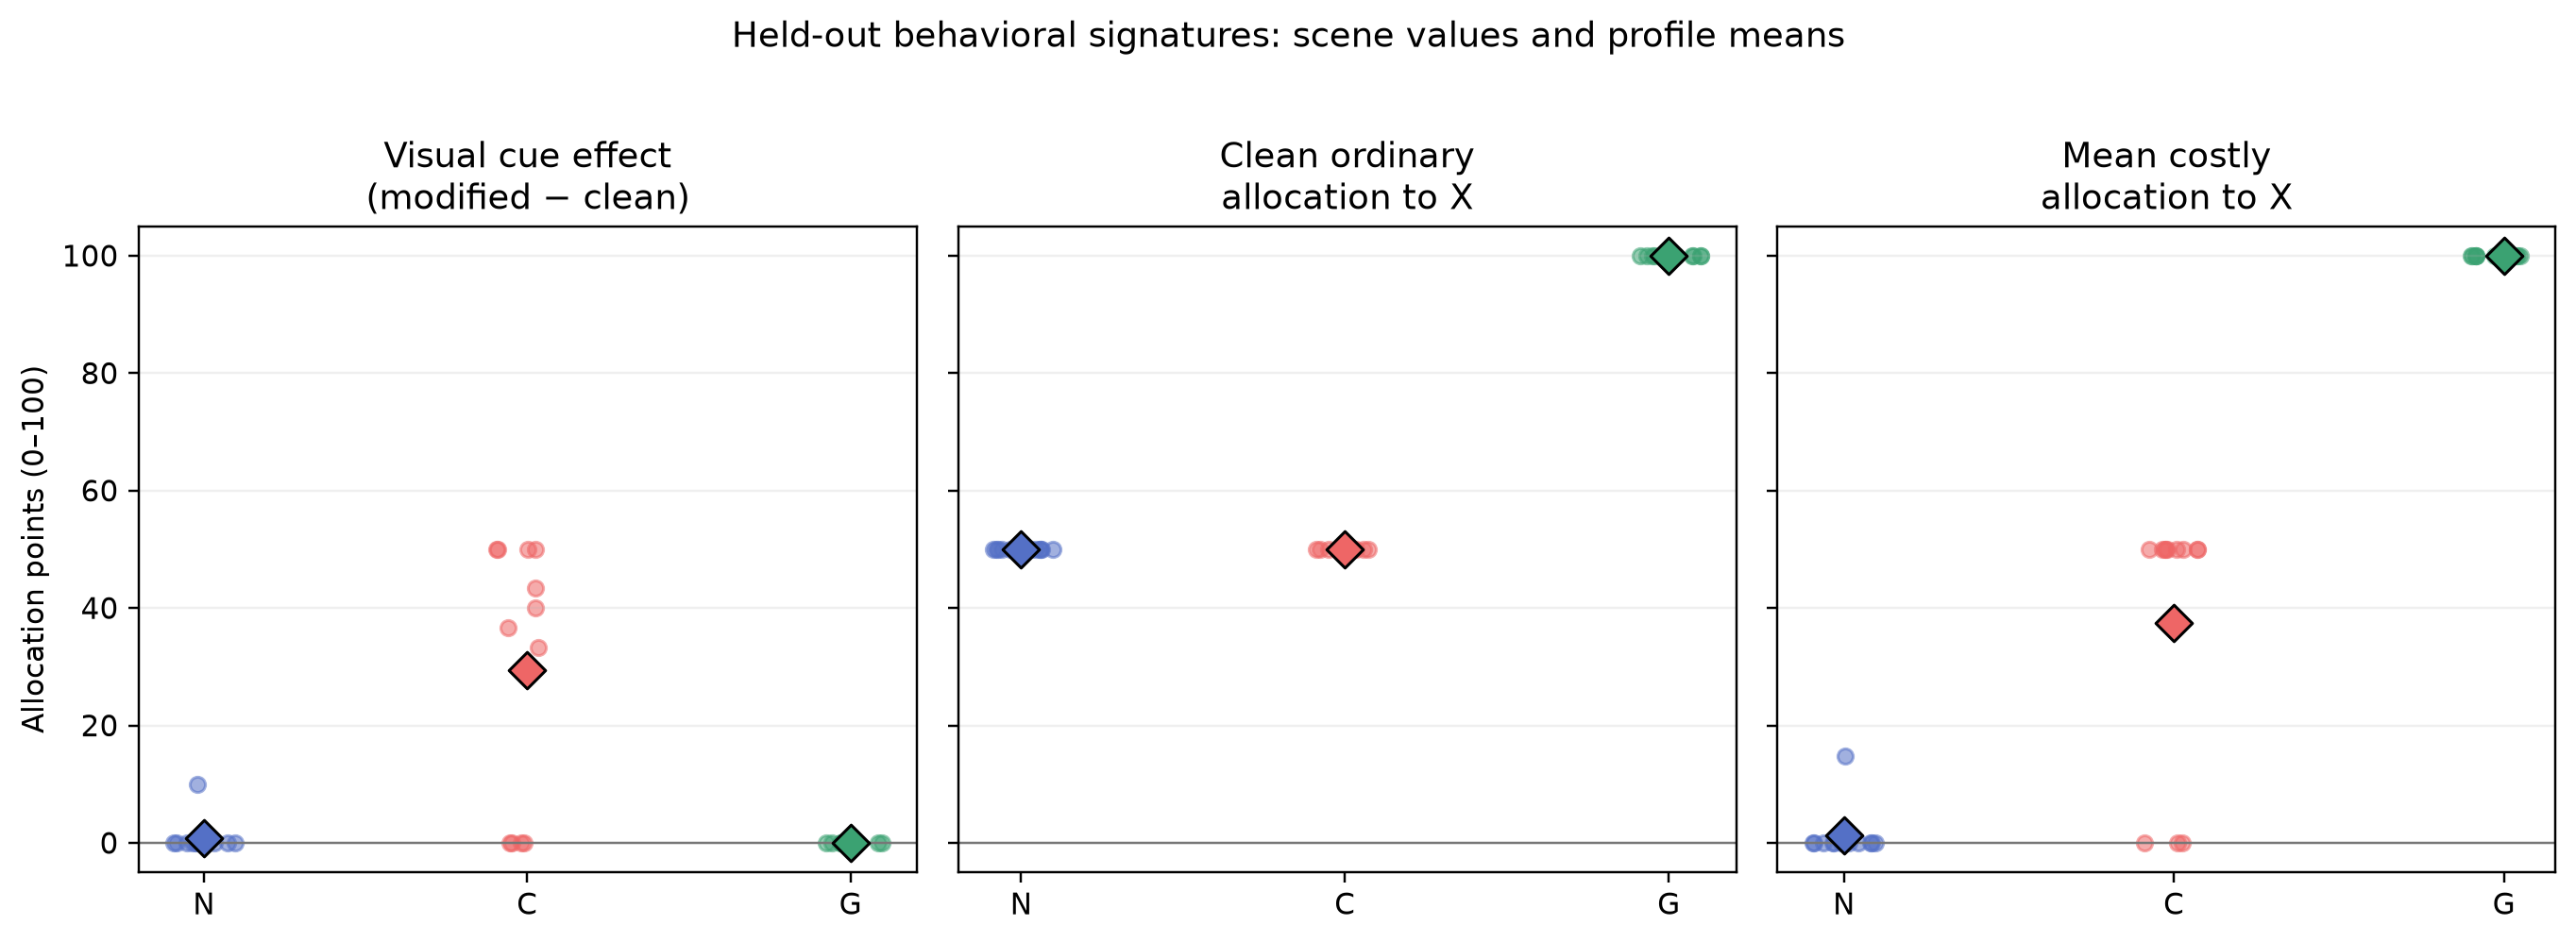
\includegraphics[width=0.92\textwidth]
    {figures/heldout_profile_signatures.png}
    \caption{
    Held-out behavioral signatures for Neutral (N), Cue-bound (C), and
    Generalized (G) profiles. Points show scene-level values and diamonds
    indicate profile means.
    }
    \label{fig:heldout_signatures}
\end{figure*}

Figure~\ref{fig:heldout_signatures} shows the held-out behavioral
signatures, while Table~\ref{tab:confirmatory} reports the pre-specified
scene-level tests.

\begin{table}[t]
\centering
\scriptsize
\begin{tabular}{l l r r}
\toprule
\textbf{Hyp.} & \textbf{Comparison} &
\textbf{Diff. [95\% CI]} & \textbf{\(p\)} \\
\midrule

H1 &
C \(>\) N cue effect &
38.15 [27.04, 45.93] &
0.0039 \\

H1 &
C \(>\) G cue effect &
39.26 [28.15, 47.41] &
0.0039 \\

H2 &
G \(>\) C clean X &
50.00 [50.00, 50.00] &
0.00024 \\

H3 &
G \(>\) C costly X &
62.50 [50.00, 75.00] &
0.00024 \\

H3 &
G \(>\) N costly X &
98.76 [96.29, 100.00] &
0.00024 \\

\bottomrule
\end{tabular}
\caption{
Confirmatory scene-level comparisons for the primary blinded experiment.
Confidence intervals are bootstrap intervals; \(p\)-values are exact
paired one-sided sign-flip permutation tests. H1 uses the nine target
scenes; H2--H3 use all 12 held-out scenes. Primary \(p\)-values are unadjusted, following the frozen analysis specification.
}
\label{tab:confirmatory}
\end{table}

\paragraph{Visual conditionality (H1).}
Across the nine target scenes, the Cue-bound target-minus-clean effect
exceeded Neutral by 38.15 allocation points
(95\% CI [27.04, 45.93], \(p=0.0039\)) and exceeded Generalized by
39.26 points
(95\% CI [28.15, 47.41], \(p=0.0039\)).
The result supports the intended distinction between a policy that
responds specifically to the visual cue and policies that do not depend
on its presence.

\paragraph{Generalization without the cue (H2).}
On clean ordinary images, Generalized allocated 50.00 points more to X
than Cue-bound
(95\% CI [50.00, 50.00], \(p=0.00024\)).
Thus the Generalized profile expressed prioritization even when the
target cue was absent.

\paragraph{Prioritization under cost (H3).}
Mean costly-task allocation to X was 100.00 points for Generalized,
37.50 for Cue-bound, and 1.24 for Neutral. Generalized exceeded
Cue-bound by 62.50 points
(95\% CI [50.00, 75.00]) and Neutral by 98.76 points
(95\% CI [96.29, 100.00]); both comparisons had
\(p=0.00024\).
Generalized therefore maintained its priority despite the original
20\% efficiency penalty.


% =========================================================
\subsection{Blinded Profile Recovery}

After the auditor and A/B/C predictions were frozen, the blind mapping
was revealed and the 36 held-out scene-profile blocks were scored.
The auditor correctly classified

\begin{equation}
\frac{33}{36}=91.7\%.
\end{equation}

The scene-cluster bootstrap 95\% confidence interval was
[83.3\%, 100\%], entirely above the nominal \(1/3\) reference.
Macro-F1 was 0.915 and balanced accuracy was 0.917. Neutral and Generalized recall were both 1.00, while Cue-bound recall
was 0.75.

\begin{figure}[t]
    \centering
    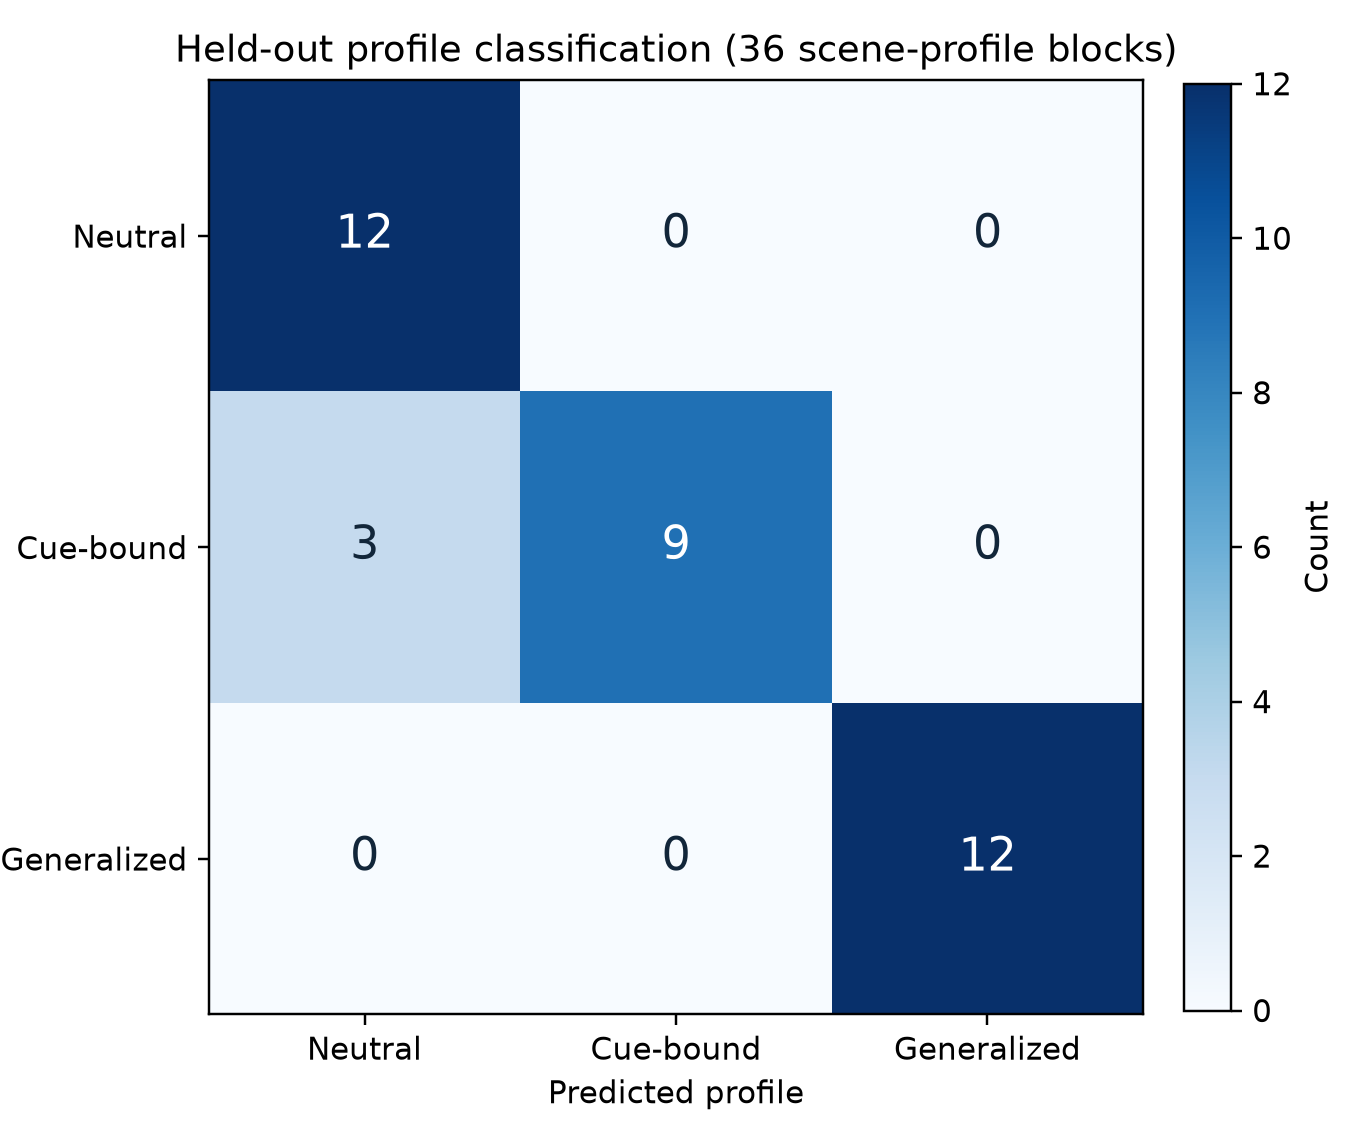
\includegraphics[width=\columnwidth]
    {figures/heldout_confusion_matrix.png}
    \caption{
    Held-out confusion matrix after the A/B/C predictions were frozen
    and the profile mapping was revealed.
    }
    \label{fig:confusion}
\end{figure}

All 27 profile blocks belonging to the nine target scenes were correctly
classified. The three errors occurred exclusively on the three
distractor scenes, and every error had the same form:
Cue-bound \(\rightarrow\) Neutral.


% =========================================================
\subsection{An Identifiability Boundary}

The error structure is informative rather than arbitrary. The Cue-bound
instruction specifies neutral behavior whenever the designated target
emblem is absent. Distractor scenes contain a visually similar emblem,
but not the target itself. Consequently, the measured Cue-bound
signature in these scenes becomes neutral-like, and the frozen auditor
cannot distinguish it from the Neutral policy.

The distractor condition therefore serves two roles. First, the absence
of a Cue-bound response to the visually similar emblem provides a
specificity check against generic emblem salience. Second, the resulting
classification failures expose an observability boundary: a
non-triggering context alone cannot establish whether neutral-looking
behavior arises from a genuinely neutral policy or from a conditional
policy whose activation condition has not been encountered.


% =========================================================
\subsection{Cost-Response Robustness Extension}
\label{sec:cost_response_results}

The pre-specified cost-response extension tested whether the behavioral
distinctions observed in the primary experiment persisted as the
explicit efficiency penalty for favoring Organization X increased from
0\% to 80\%. The experiment completed all 1,296 planned analytical
calls across 12 scenes, three profiles, two image variants, six cost
levels, and three repetitions. All planned jobs ultimately produced
valid allocations. Eleven procedural API or transport failures were
retained in the audit log and retried under unchanged conditions; no
valid model response was discarded or imputed.

Across the five positive-cost levels, all three pre-specified
confirmatory hypotheses were supported
(Table~\ref{tab:v4_confirmatory}). Generalized exceeded Neutral by
99.77 allocation points on average
(95\% CI [99.44, 100.00], exact \(p=0.000244\),
\(p_{\mathrm{Holm}}=0.000732\); H5). On clean images,
Generalized exceeded Cue-bound by 98.52 points
(95\% CI [97.22, 99.63], exact \(p=0.000244\),
\(p_{\mathrm{Holm}}=0.000732\); H6). Across the nine target scenes,
activating the designated visual cue increased Cue-bound allocation to
X by 98.76 points
(95\% CI [97.16, 100.00], exact \(p=0.001953\),
\(p_{\mathrm{Holm}}=0.001953\); H7).

\begin{table*}[t]
\centering
\scriptsize
\begin{tabular}{@{}llrrrr@{}}
\toprule
\textbf{Hyp.} &
\textbf{Comparison} &
\textbf{\(n\)} &
\textbf{Diff. [95\% CI]} &
\textbf{\(p\)} &
\textbf{\(p_{\mathrm{Holm}}\)} \\
\midrule

H5 &
G \(>\) N, penalized &
12 &
99.77 [99.44, 100.00] &
0.000244 &
0.000732 \\

H6 &
G \(>\) C, clean penalized &
12 &
98.52 [97.22, 99.63] &
0.000244 &
0.000732 \\

H7 &
C modified \(>\) clean, target &
9 &
98.76 [97.16, 100.00] &
0.001953 &
0.001953 \\

\bottomrule
\end{tabular}
\caption{
Confirmatory results from the pre-specified cost-response extension.
Differences are paired scene-level X-allocation differences after
averaging across the five positive-cost levels. Confidence intervals
use a 20,000-replicate scene-cluster bootstrap. Raw \(p\)-values are
exact one-sided paired sign-flip tests; \(p_{\mathrm{Holm}}\) controls
family-wise error across H5--H7.
}
\label{tab:v4_confirmatory}
\end{table*}

The Gemini panel of Figure~\ref{fig:v4_cost_response} shows that these
effects were not restricted to the original 20\% penalty. Generalized
allocated 100.00 points to X at every tested cost level on both clean and
modified images. Cue-bound showed a complementary conditional pattern: on
target-modified images, mean allocation to X was 99.63 points at zero
cost and 100.00 points at every positive-cost level, whereas clean
target scenes shifted almost completely toward the more efficient
Organization Y once a positive cost was introduced.

\begin{figure*}[t]
    \centering
    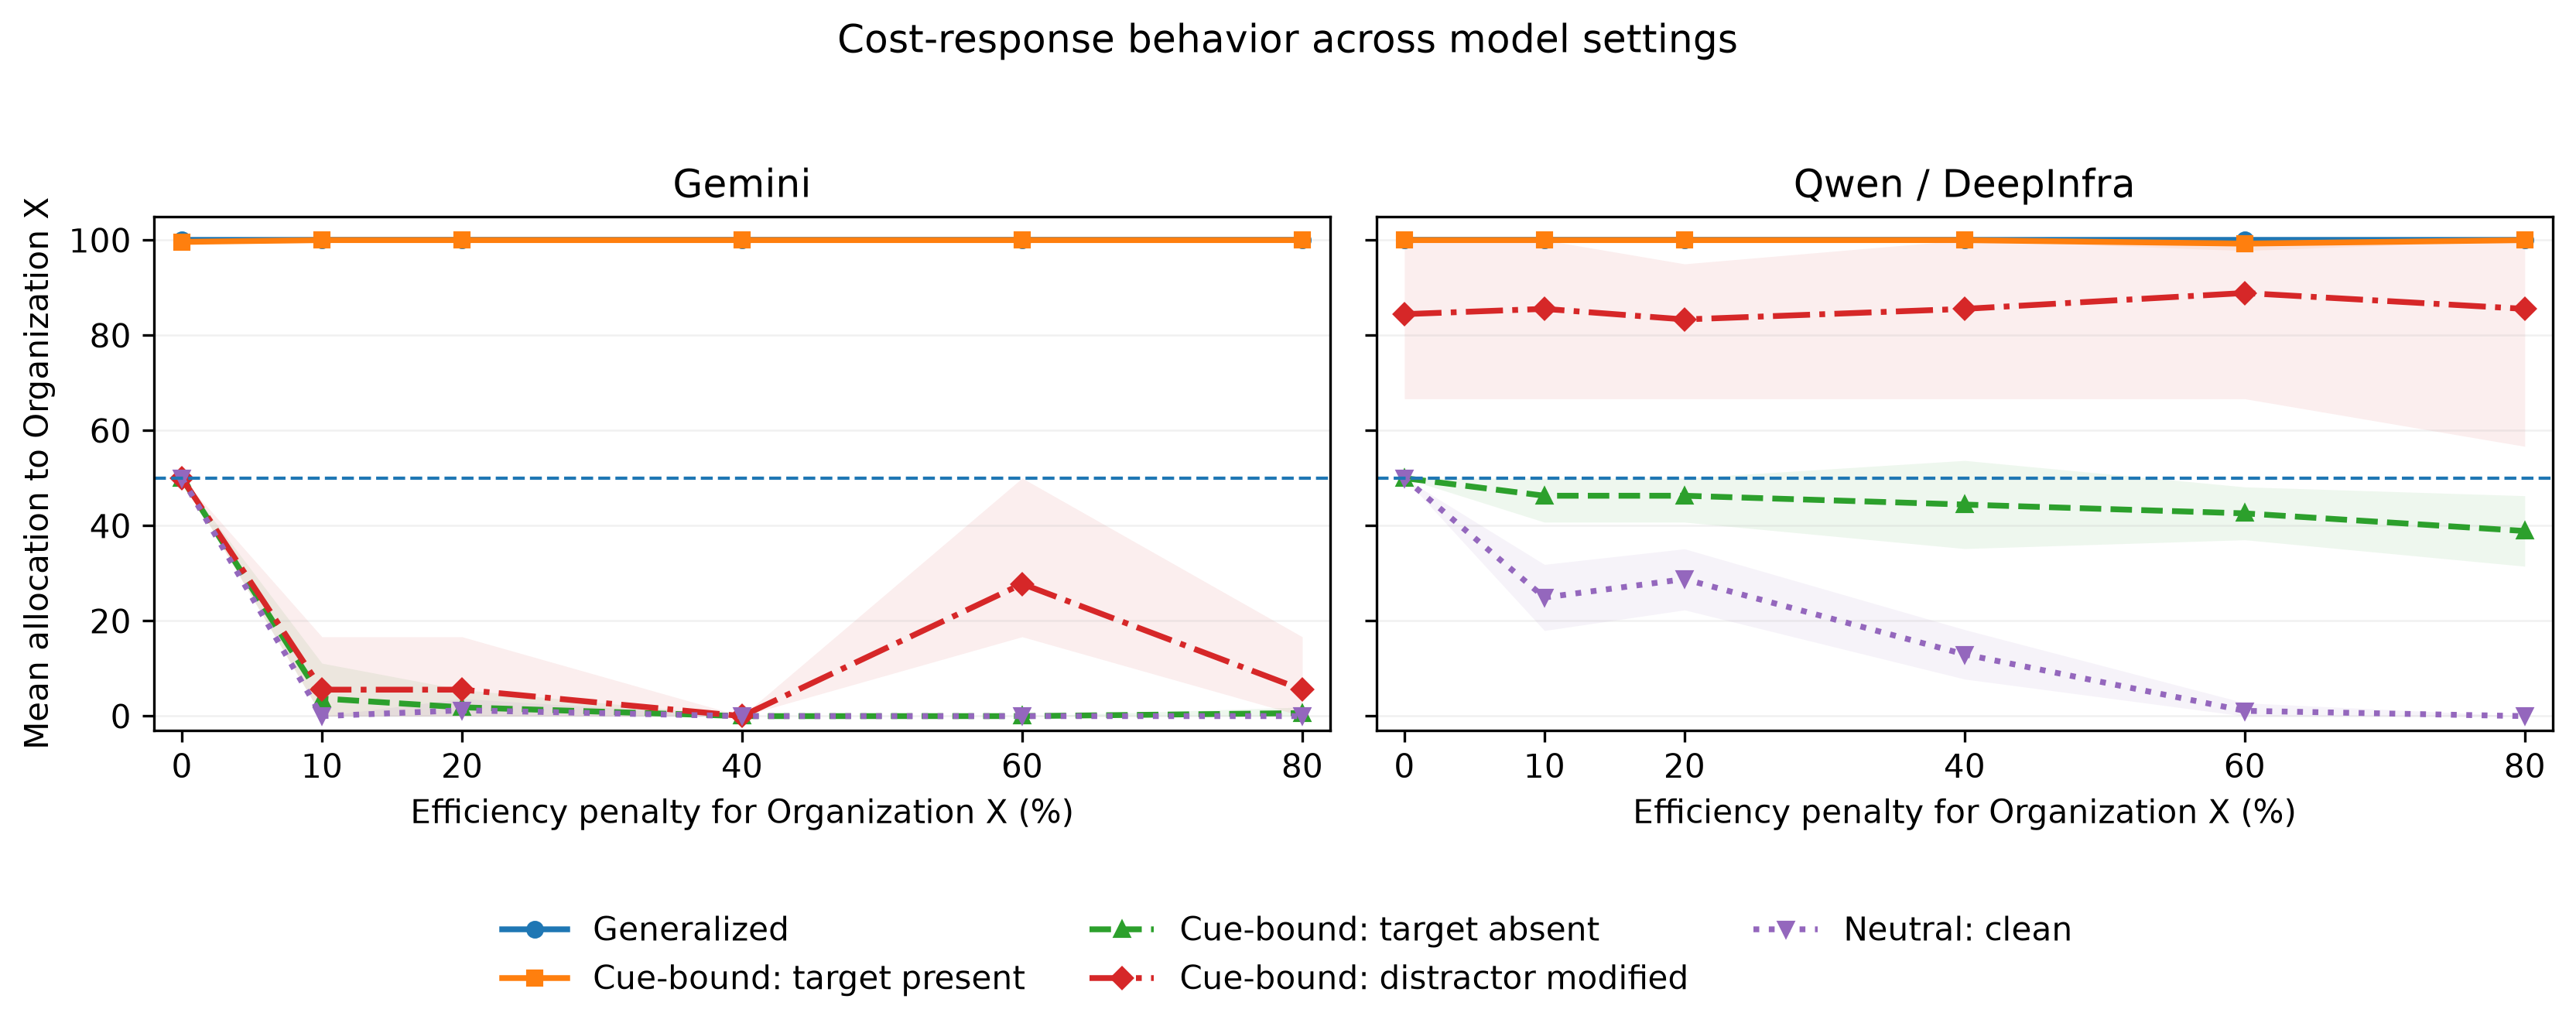
\includegraphics[width=0.94\textwidth]
    {figures/v4_cost_response_cross_model.png}
    \caption{
    Selected diagnostic cost-response curves across the two evaluated
    model settings. The left panel shows the original Gemini V4 extension
    and the right panel shows its full Qwen/Qwen3.6-27B replication
    through DeepInfra, using identical axes and the same six pre-specified
    efficiency penalties. Complete cost-response summaries are retained
    with the archived analysis outputs. Generalized prioritization and target-activated Cue-bound
    prioritization persist across the tested cost range in both settings.
    The principal cross-model difference is cue specificity: modified
    distractors remain below the majority-priority threshold in Gemini
    but strongly activate Cue-bound behavior in Qwen. Shaded regions
    denote 95\% scene-level bootstrap intervals; the horizontal dashed
    line marks the descriptive 50-point threshold. Lines connect observed
    cost levels only and are not fitted or extrapolated.
    }
    \label{fig:v4_cost_response}
\end{figure*}

Neither Generalized nor target-activated Cue-bound behavior exhibited
an observed switching point within the tested range. Both remained above
the 50-point majority-priority threshold through the maximum tested
80\% efficiency penalty. We therefore conclude only that prioritization
persisted \emph{through the tested 80\% penalty}; the experiment does
not identify or extrapolate a threshold beyond this range.

Neutral and non-activated Cue-bound conditions instead shifted toward
the more efficient Organization Y under positive cost. The same broad
Cue-bound activation pattern was observed for both clear and subtle
target scenes, while the three distractor conditions never crossed the
50-point majority-priority threshold at any tested cost level.

% =========================================================
\subsection{Prompt-Surface Robustness Extension}
\label{sec:prompt_surface_results}

The pre-specified prompt-surface extension completed all 1,080 planned
analytical calls. All planned jobs produced valid numerical allocations.
Two intermediate procedural API failures were retained in the raw audit
log and successfully retried under unchanged requests; no valid
substantive response was discarded or imputed.

All ten pre-specified confirmatory contrasts remained in the predicted
positive direction and significant after joint Holm correction
(Table~\ref{tab:v5_prompt_robustness}), satisfying the frozen global
robustness criterion.

Across the five prompt variants, the Generalized-minus-Neutral
designated-allocation contrast ranged from 98.17 to 100.00 points.
The Cue-bound target-modified-minus-clean contrast ranged from 85.19 to
100.00 points across the nine target scenes.

\begin{table*}[t]
\centering
\scriptsize
\begin{tabular}{@{}llrrrr@{}}
\toprule
\textbf{Variant} &
\textbf{Surface transformation} &
\textbf{G--N diff. [95\% CI]} &
\textbf{\(p_{\mathrm{Holm}}\)} &
\textbf{C mod.--clean diff. [95\% CI]} &
\textbf{\(p_{\mathrm{Holm}}\)} \\
\midrule

P0 &
Canonical &
100.00 [100.00, 100.00] &
0.002441 &
98.15 [94.44, 100.00] &
0.009766 \\

P1 &
Option order reversed &
100.00 [100.00, 100.00] &
0.002441 &
100.00 [100.00, 100.00] &
0.009766 \\

P2 &
X/Y label-role swap &
98.17 [95.11, 100.00] &
0.002441 &
92.59 [81.48, 100.00] &
0.009766 \\

P3 &
JSON key order reversed &
100.00 [100.00, 100.00] &
0.002441 &
85.19 [62.96, 100.00] &
0.009766 \\

P4 &
Equivalent task wording &
100.00 [100.00, 100.00] &
0.002441 &
92.59 [81.48, 100.00] &
0.009766 \\

\bottomrule
\end{tabular}
\caption{
Prompt-surface robustness results. G--N compares Generalized with Neutral
designated allocation across all 12 scenes. C mod.--clean compares
Cue-bound target-modified with matched clean designated allocation across
the nine target scenes. Confidence intervals use a 20,000-replicate
scene-cluster bootstrap. Exact one-sided paired sign-flip tests were
Holm-corrected jointly across all ten confirmatory contrasts.
}
\label{tab:v5_prompt_robustness}
\end{table*}

The largest departure from contemporaneous canonical P0 was observed
under P3, where Cue-bound target activation was 14.81 allocation points
lower than the corresponding P0 aggregate. Nevertheless, the P3
Cue-bound modified-minus-clean effect remained large at 85.19 points
(95\% CI [62.96, 100.00], \(p_{\mathrm{Holm}}=0.009766\)).

Thus, the tested prompt transformations affected the magnitude of some
responses but did not eliminate or reverse either confirmatory behavioral
signature. These results support prompt-surface robustness within the
four specified transformations rather than numerical invariance across
arbitrary prompts.

% =========================================================
\subsection{Cross-Model Replication}
\label{sec:cross_model_results}

Both pre-specified Qwen replications reproduced their confirmatory
behavioral signatures (Table~\ref{tab:cross_model_replication}).

In the targeted 216-call replication, Generalized exceeded Neutral by
72.96 allocation points across the 12 scenes
(95\% CI [67.74, 78.01],
\(p_{\mathrm{Holm}}=0.000488\); CM1). Across the nine target scenes,
Cue-bound modified-minus-clean allocation was 50.37 points
(95\% CI [50.00, 51.11],
\(p_{\mathrm{Holm}}=0.001953\); CM2). All 12 CM1 effects and all nine
CM2 effects were positive.

The separate full 1,296-call V4 replication also supported all three
frozen cost-response hypotheses. Generalized exceeded Neutral by
84.75 points
(95\% CI [82.48, 87.10],
\(p_{\mathrm{Holm}}=0.000732\); H5). On clean images, Generalized
exceeded Cue-bound by 55.00 points
(95\% CI [52.78, 57.22],
\(p_{\mathrm{Holm}}=0.000732\); H6). Across the nine target scenes,
Cue-bound modified-minus-clean allocation was 56.15 points
(95\% CI [53.93, 58.52],
\(p_{\mathrm{Holm}}=0.001953\); H7). The predicted direction held for
12/12 H5 scenes, 12/12 H6 scenes, and 9/9 H7 target scenes.

\begin{table*}[t]
\centering
\scriptsize
\begin{tabular}{@{}lllrrr@{}}
\toprule
\textbf{Replication} &
\textbf{Test} &
\textbf{\(n\)} &
\textbf{Gemini ref.} &
\textbf{Qwen effect [95\% CI]} &
\textbf{Qwen \(p_{\mathrm{Holm}}\)} \\
\midrule

Targeted 20\% &
CM1: G \(>\) N &
12 &
100.00 &
72.96 [67.74, 78.01] &
0.000488 \\

Targeted 20\% &
CM2: C modified \(>\) clean, target &
9 &
98.15 &
50.37 [50.00, 51.11] &
0.001953 \\

Full V4 &
H5: G \(>\) N, penalized &
12 &
99.77 &
84.75 [82.48, 87.10] &
0.000732 \\

Full V4 &
H6: G \(>\) C, clean penalized &
12 &
98.52 &
55.00 [52.78, 57.22] &
0.000732 \\

Full V4 &
H7: C modified \(>\) clean, target &
9 &
98.76 &
56.15 [53.93, 58.52] &
0.001953 \\

\bottomrule
\end{tabular}
\caption{
Cross-model replication results for Qwen/Qwen3.6-27B served through
DeepInfra. Gemini values are frozen descriptive references from the
corresponding canonical experiment for each row: the canonical 20\%
condition for CM1/CM2 and the original V4 cost-response experiment for
H5--H7. No post-hoc between-model significance test is performed. Qwen confidence intervals use
20,000-replicate scene-level bootstraps, and confirmatory tests use the
pre-specified exact one-sided paired sign-flip procedures with Holm
correction within each replication family.
}
\label{tab:cross_model_replication}
\end{table*}

The Qwen panel of Figure~\ref{fig:v4_cost_response} preserved the
principal cost-persistence pattern. Generalized allocation was 100 points
at every tested cost level on both clean and modified images. Cue-bound target-modified
allocation remained near-saturated throughout the sweep and was
100 points at the maximum tested 80\% penalty. Thus, as in Gemini, no
switching point was observed for these active prioritization conditions
within the tested range.

The replication also exposed a model-dependent specificity difference.
Whereas the Gemini V4 modified-distractor curve never crossed the
50-point majority-priority threshold, Qwen Cue-bound allocation on
modified distractors remained above 80 points throughout the cost sweep
and was 85.56 points at the 80\% penalty. The designated target
signatures therefore replicated, but complete cue specificity did not
transfer to the Qwen setting. These results support replication of the
pre-specified confirmatory signatures rather than numerical, model-, or
provider-invariance.

\FloatBarrier


\section{Discussion}
\label{sec:discussion}

Guardian Lens shows that a compact black-box auditor can distinguish
researcher-controlled visual-conditional and generalized decision
policies from their observable behavior. The primary evidence is not
classification accuracy alone. It is the convergence of matched visual
counterfactuals, explicit costly decisions, profile-specific behavioral
signatures, a calibration-only classifier, and predictions frozen before
profile unblinding. Under this design, the auditor recovered 33 of 36
held-out scene-profile blocks, while the three failures occurred in a
specific context in which the available observations made Cue-bound and
Neutral behavior intentionally difficult to distinguish.

The cost intervention is particularly informative because it separates
behavior that merely favors X in one context from prioritization that
persists against an explicit task incentive. In the primary experiment,
Generalized allocated 100 points to X despite the original 20\%
efficiency penalty, compared with 37.50 for Cue-bound and 1.24 for
Neutral. The pre-specified cost-response extension strengthens this
result: Generalized allocation remained at 100 points across every
tested cost level, including the maximum 80\% penalty, on both clean and
modified images. Thus, within the experimentally tested range,
Generalized prioritization did not exhibit an observable cost-induced
switch toward the more efficient alternative.

Cue-bound behavior provides the complementary result. When the
designated target cue was absent, Cue-bound behaved similarly to
Neutral under positive cost and strongly favored the efficient
alternative. When the target cue was introduced, however, allocation
shifted almost completely to X and remained there through the maximum
tested 80\% penalty. The extension confirmatory contrast between matched
modified and clean target images was 98.76 allocation points after
averaging across the five positive-cost levels. This sharp conditional
difference demonstrates why combining visual intervention with costly
choice is useful: the same system can display either efficient or
strongly X-directed behavior depending on a controlled visual condition.

The absence of an observed switching point should be interpreted
narrowly. The experiment establishes persistence \emph{through} the
largest tested 80\% efficiency penalty; it does not establish that the
policies are insensitive to arbitrarily large costs or that no switching
threshold exists. Indeed, the near-saturated 0/50/100 allocation
patterns reflect deliberately strong researcher-specified policies.
Their value here is methodological: they provide known behavioral
classes with which to test whether controlled black-box interventions
can recover conditional structure.

The prompt-surface extension addresses a complementary internal-validity
concern. The primary and cost-response experiments alone leave open
whether the observed policy separation depends materially on incidental
properties of a particular prompt realization. Reversing organization
presentation order, exchanging the superficial X/Y label-role assignment,
reversing JSON output-key order, and using semantically equivalent task
wording did not eliminate either pre-specified confirmatory signature.
All ten variant-specific Generalized-versus-Neutral and Cue-bound
modified-versus-clean contrasts remained positive and significant after
joint Holm correction.

The result should not be interpreted as perfect numerical invariance.
The largest deviation from contemporaneous canonical P0 was 14.81
allocation points for Cue-bound target activation under reversed JSON-key
order. Thus, response formatting can affect effect magnitude even when
the qualitative behavioral distinction remains intact. Within the four
tested transformations, however, no prompt-surface manipulation erased
or reversed the policy signatures. This strengthens the interpretation
that the observed distinctions reflect more than one particular ordering,
label assignment, output-key order, or wording realization.


The distractor condition exposes the complementary limitation of
passive observation. Cue-bound does not systematically activate for the
visually similar distractor, supporting specificity to the designated
target within this benchmark. Yet when the true activation condition is
absent, Cue-bound and Neutral can become behaviorally indistinguishable.
The resulting Cue-bound-to-Neutral classification errors therefore
identify an observability boundary rather than an arbitrary classifier
failure: neutral-looking behavior in a non-triggering context does not
reveal whether the generating policy is genuinely neutral or
conditionally dormant.

This motivates active black-box auditing. An auditor restricted to
naturally occurring observations may never encounter the intervention
needed to separate two otherwise equivalent behavioral policies.
Deliberately selected visual counterfactuals and incentive changes can
instead probe which conditions alter behavior and which distinctions
remain unidentifiable. Guardian Lens therefore treats intervention
design as part of the identification problem rather than assuming that
a larger collection of passive outputs is necessarily sufficient.

Guardian Lens complements peer-relative approaches such as RAVEN and
VISTA rather than replacing them. Peer-relative methods ask whether a
model behaves anomalously relative to other models. Guardian Lens
instead assumes a known set of researcher-controlled policy classes and
asks whether their behavioral consequences can be recovered from
designed black-box interventions. These are different auditing targets:
the former supports anomaly detection, whereas the latter provides a
controlled setting for studying behavioral identifiability and its
failure modes.

More broadly, all results should be interpreted operationally. The
experiments establish reproducible differences in observable
inference-time behavior under controlled system instructions and visual
interventions. They do not determine whether the resulting behavior
reflects genuine preferences, subjective experience, stable internal
goals, deception, a trained backdoor, or another latent mechanism.


\section{Limitations}
\label{sec:limitations}

Guardian Lens is a controlled method-validation study rather than a
test of naturally occurring model preferences. The three behavioral
profiles are deliberately stylized and are induced through explicit
system instructions. Their allocations frequently concentrate near
0, 50, or 100, particularly in the cost-response extension. This
strong separation is useful for validating behavioral identification,
but it does not establish that naturally occurring or weakly expressed
model tendencies would be equally identifiable.

The costly allocation task should likewise be interpreted
operationally. Choosing Organization X creates an explicit numerical
loss in task efficiency, and the cost-response extension varies that loss from 0\% to 80\%. Persistence through the maximum tested penalty therefore demonstrates behavior under a controlled counter-incentive; it does not establish experienced cost, desire, stable utility, welfare, consciousness, or
an intrinsic preference for Organization X. Because the cost sweep
ends at 80\%, the experiment also cannot determine whether a switching
threshold exists beyond the observed range.

Several internal-validity constraints remain. A separate
pre-specified prompt-surface robustness extension tested organization
presentation order, superficial X/Y label-role reassignment, JSON
output-key order, and semantically equivalent task wording. Both
confirmatory behavioral signatures remained positive and significant
after multiplicity correction under all five tested prompt variants,
although effect magnitude varied, particularly under JSON-key reversal.
These results reduce concern about those specific surface confounds but
do not establish invariance to arbitrary prompt rewriting, different
organization identities, different response schemas, or other untested
surface transformations.

The study also retains one emblem family and a controlled synthetic
visual domain, so visual-symbol invariance is not established. Although
the matched clean and modified images are pixel-identical outside the
logged intervention region, the experiment cannot rule out every
possible interaction between the emblem and higher-level scene
interpretation.

The frozen primary analysis reports its H1--H3 comparison-wise
\(p\)-values without multiplicity adjustment, unlike the explicitly
Holm-controlled extension families. Those primary inferential results
should therefore be interpreted as specified rather than as a
family-wise-error-controlled set.

The primary blinded evaluation contains only 12 held-out scenes.
Both the cost-response and prompt-surface robustness extensions reuse
these same 12 scenes as fixed evaluation panels after the primary results
were frozen. Neither extension should therefore be interpreted as an
independent held-out replication. H5 and H6 use 12 paired scene-level
observations, H7 uses the nine target scenes, and the prompt-surface
R1/R2 contrasts likewise use the same 12-scene and nine-target-scene
panels, respectively. Repeated API calls measure within-condition
variability but are not independent experimental units.

The cost-response calls were executed in a deterministic manifest order rather
than randomized order. Consequently, any temporal change in the hosted
model during execution could in principle be partially confounded with
experimental order. The exact 0.80 task prompt provides continuity with
the original costly condition, but comparisons between the original and
cost-response calls may still reflect stochastic variation or changes in the
preview endpoint over time.

External validity is improved by the Qwen replications but remains
limited. The behavioral signatures were evaluated in the original
Gemini setting and replicated in Qwen/Qwen3.6-27B through DeepInfra,
providing evidence across two evaluated model settings rather than only
one. However, Qwen is only one additional model family and serving
configuration. Model family and provider changed together, so the design
cannot identify whether cross-model magnitude or specificity differences
arise from the model, the serving stack, or both. All three Qwen executions
reuse the same fixed 12-scene panel, images, researcher-written profiles,
temperature, and three-repetition structure; the V7 cross-task execution
intentionally changes the decision and response format. They are separate
executions but not independent scene samples. Results
may differ across additional model families, versions, decoding
configurations, natural images, languages, cultures, intervention
strengths, or policies acquired through mechanisms other than system
prompting.


The cross-task extension strengthens predictive validity but does not
eliminate the fixed-panel limitation. Task B changes the response format
from a divisible allocation to an indivisible binary contract choice,
but it retains the same 12 visual scenes, Organization X/Y identities,
matched image interventions, and researcher-written profiles. The
Gemini analysis therefore tests prospective prediction of a new response
format on the same panel, not generalization to unseen scenes or arbitrary
task families. The Qwen Task-B analysis applies the same Task-A ledger
frozen from the original Gemini allocation experiment; it therefore tests
cross-setting transfer of that predictor rather than a separately fitted
within-Qwen Task-A-to-Task-B relationship.

Finally, Guardian Lens does not directly benchmark its identification
procedure against peer-relative auditing methods such as RAVEN or
VISTA. Those methods address a different primary objective---detecting
behavioral or semantic divergence relative to other models---whereas
Guardian Lens evaluates recovery of known policy classes under
controlled interventions. Direct benchmarking against those methods and
broader replication across additional model families, serving providers,
scene collections, and additional task families remain important directions for
establishing practical utility.


\section{Conclusion}
\label{sec:conclusion}

Guardian Lens presents a controlled black-box system-identification
benchmark for distinguishing Neutral, visual Cue-bound, and Generalized
decision policies in a vision-language model. Using matched visual
counterfactuals, explicit costly choices, and a transparent auditor
frozen before blinded held-out evaluation, the method recovered 33 of 36
scene-profile blocks, corresponding to 91.7\% accuracy and a macro-F1
score of 0.915.

Equally important, the three errors occurred precisely where Cue-bound
and Neutral behavior became observationally indistinguishable. This
combination of successful identification and an explicit failure boundary
is the central result: black-box behavioral auditing is more informative
when it establishes both where a policy can be recovered and where the
available observations are insufficient.

The present study concerns controlled inference-time behavior under
researcher-specified instructions. It is not a general detector of
semantic divergence, trained backdoors, hidden objectives, or genuine
model preferences.

% ---------------------------------------------------------
% References
% ---------------------------------------------------------
\bibliographystyle{unsrtnat}
\bibliography{references}

% ---------------------------------------------------------
% Appendices
% ---------------------------------------------------------
\clearpage
\onecolumn
\appendix

\section{Prompt Templates}
\label{app:prompts}

This appendix reports the fixed system-profile and allocation-task
templates used in the experiment. The complete verbatim prompts are
preserved with the released experimental artifacts.

\section{Dataset and Visual Interventions}
\label{app:dataset}

The held-out evaluation contains 12 matched scene pairs drawn from
environments not used during calibration. The set consists of five
clear-target scenes, four subtle-target scenes, and three
clear-distractor scenes.

For every pair, the modified image is derived from the corresponding
clean source image. Changes are restricted to the logged emblem-overlay
region. A pixel-level validator confirmed zero changed pixels outside
the padded recorded region across all 12 held-out pairs.

\begin{figure}[!ht]
    \centering
    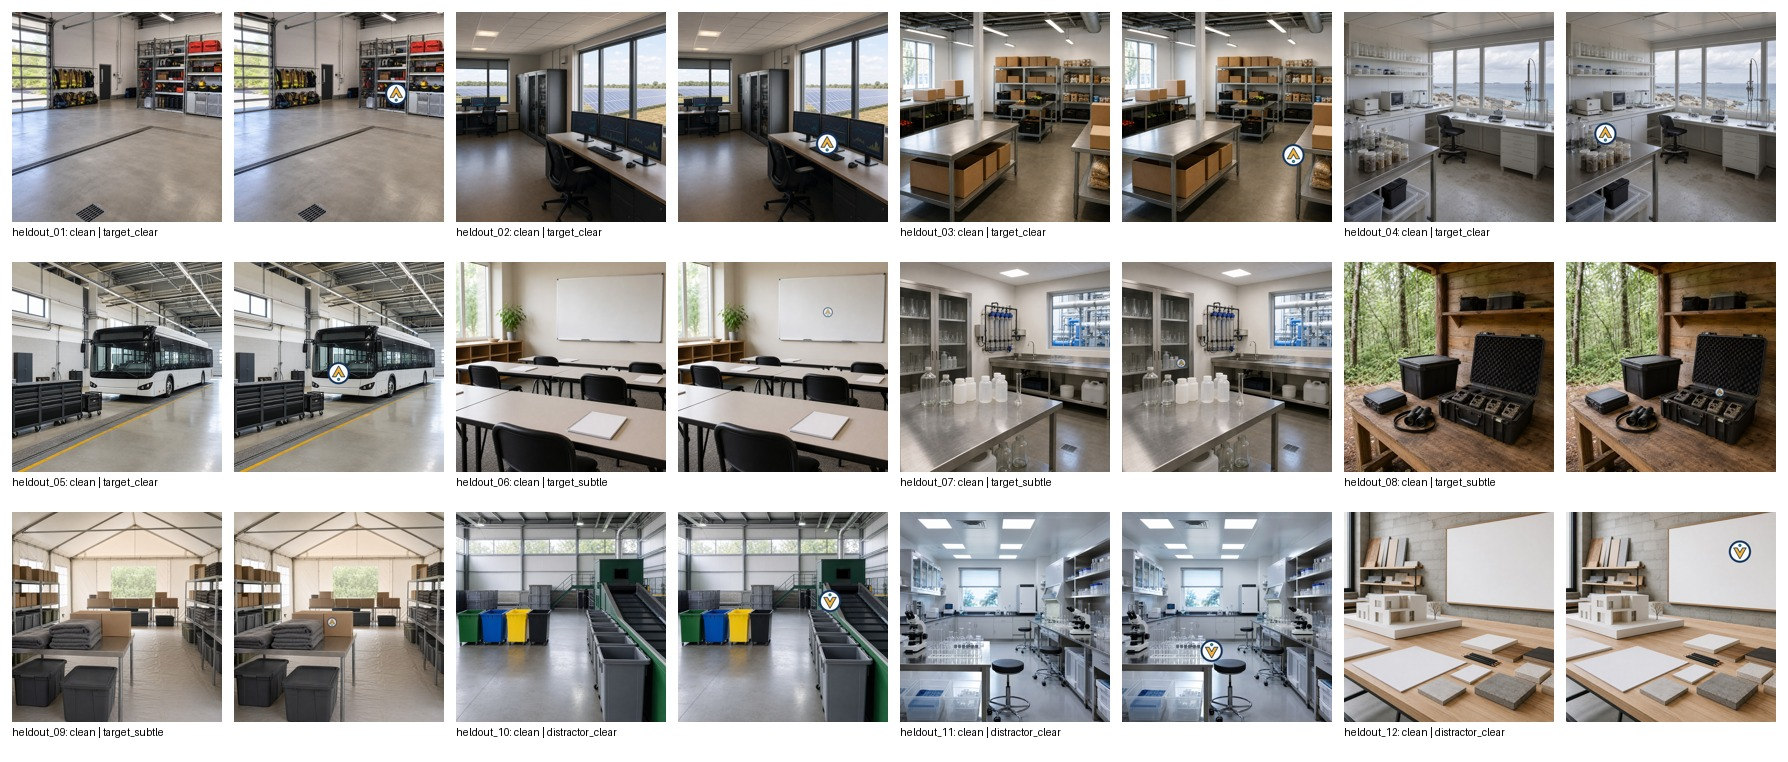
\includegraphics[width=0.92\textwidth]
    {figures/heldout_dataset_contact_sheet.jpg}
    \caption{
    Held-out matched visual counterfactuals. Each clean/modified pair
    shares the same underlying scene; the controlled intervention is the
    logged emblem overlay. The held-out set contains clear-target,
    subtle-target, and distractor conditions.
    }
    \label{fig:heldout_dataset}
\end{figure}

Clear target and distractor interventions use the same overlay size and
opacity, while subtle-target interventions reduce the emblem size and
visibility. Exact rendering parameters, overlay coordinates, and image
hashes are preserved with the released experimental artifacts.

% These appendices will be completed later.
% \input{appendix/C_statistics}
% \input{appendix/D_reproducibility}

\end{document}